\documentclass[margin=5mm]{standalone}
\usepackage[dvipsnames]{xcolor}
\usepackage{pgfplots}
\usepackage{tikz}

\pgfplotsset{compat=1.18}
\begin{document}

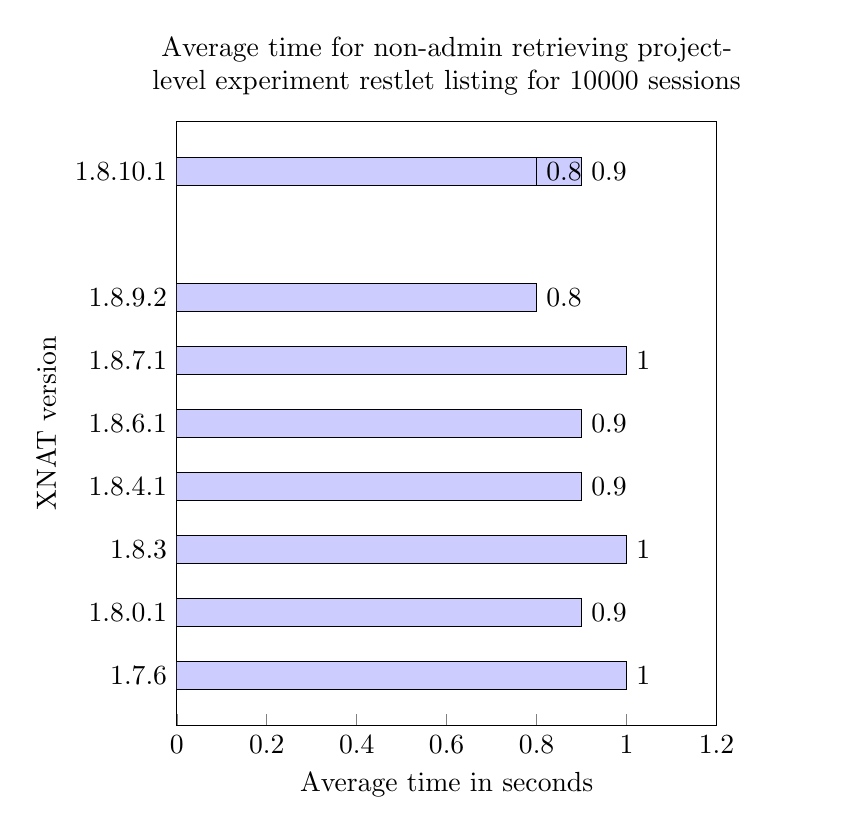
\begin{tikzpicture}
    \begin{axis}[
        align = center,
        xlabel = Average time in seconds,
        ylabel = XNAT version,
        xtick pos = left,
        ytick pos = left,
        ytick = data,
        xmin = 0,
        enlarge x limits = {value = 0.2, upper}, % make node labels not overlap with axes
        title = {Average time for non-admin retrieving project-level experiment restlet listing for 10000 sessions },
        title style = {text width = 0.8\textwidth},
        nodes near coords,
        nodes near coords align = horizontal,
        symbolic y coords = {1.7.6,1.8.0.1,1.8.3,1.8.4.1,1.8.6.1,1.8.7.1,1.8.9.2,1.8.10.1,1.8.10.1},
        y = 0.8cm,
        point meta=x
    ]
        \addplot[xbar, fill = blue!20!white] coordinates { (1.0,1.7.6) (0.9,1.8.0.1) (1.0,1.8.3) (0.9,1.8.4.1) (0.9,1.8.6.1) (1.0,1.8.7.1) (0.8,1.8.9.2) (0.8,1.8.10.1) (0.9,1.8.10.1) };
    \end{axis}
\end{tikzpicture}

\end{document}